% Peter Westerbaan
\documentclass[landscape]{article}
\usepackage[margin=1in,landscape]{geometry}
\usepackage{fancyhdr}
\usepackage{tikz}
\usetikzlibrary{fit, positioning, arrows, backgrounds, calc, shapes}
%----------------------------------------------------------------
\pagestyle{fancy}
\fancyhf{}
\lhead{
  \tikz[baseline=-0.75ex]{\draw[arrow](0,0) -- (1,0);}\ Prerequisite\\
  Modified: \today}
\chead{\huge \textbf{MTHSC Course Dependencies}}
\rhead{\vspace*{-20pt}
  \tikz{\node[class, double]{Breadth Course};}\\
  \underline{Prelim Course} 
}
\renewcommand{\headrulewidth}{2pt}
%----------------------------------------------------------------
% nodes for classes. 
% Add option 'double' for breadth course
% Underline number for prelim course
% Draw arrows for dependencies after both nodes are drawn.
\tikzstyle{class} = [rectangle, 
    fill=white,
    rounded corners, 
    minimum width=35pt, 
    minimum height=20pt,
    text centered, 
    draw=black] 

\tikzstyle{subject}=[draw=black, 
    dashed, 
    rounded corners, 
    fill=black!05]

\tikzstyle{arrow} = [thick,->,>=stealth]
%----------------------------------------------------------------
\begin{document}
  \vspace*{\fill}
  \center
  \large
  \def\nodeHt{17.5pt} %vert  distance between nodes
  \def\nodeWt{12.5pt} %horiz distance (for diagonals)
  \center
  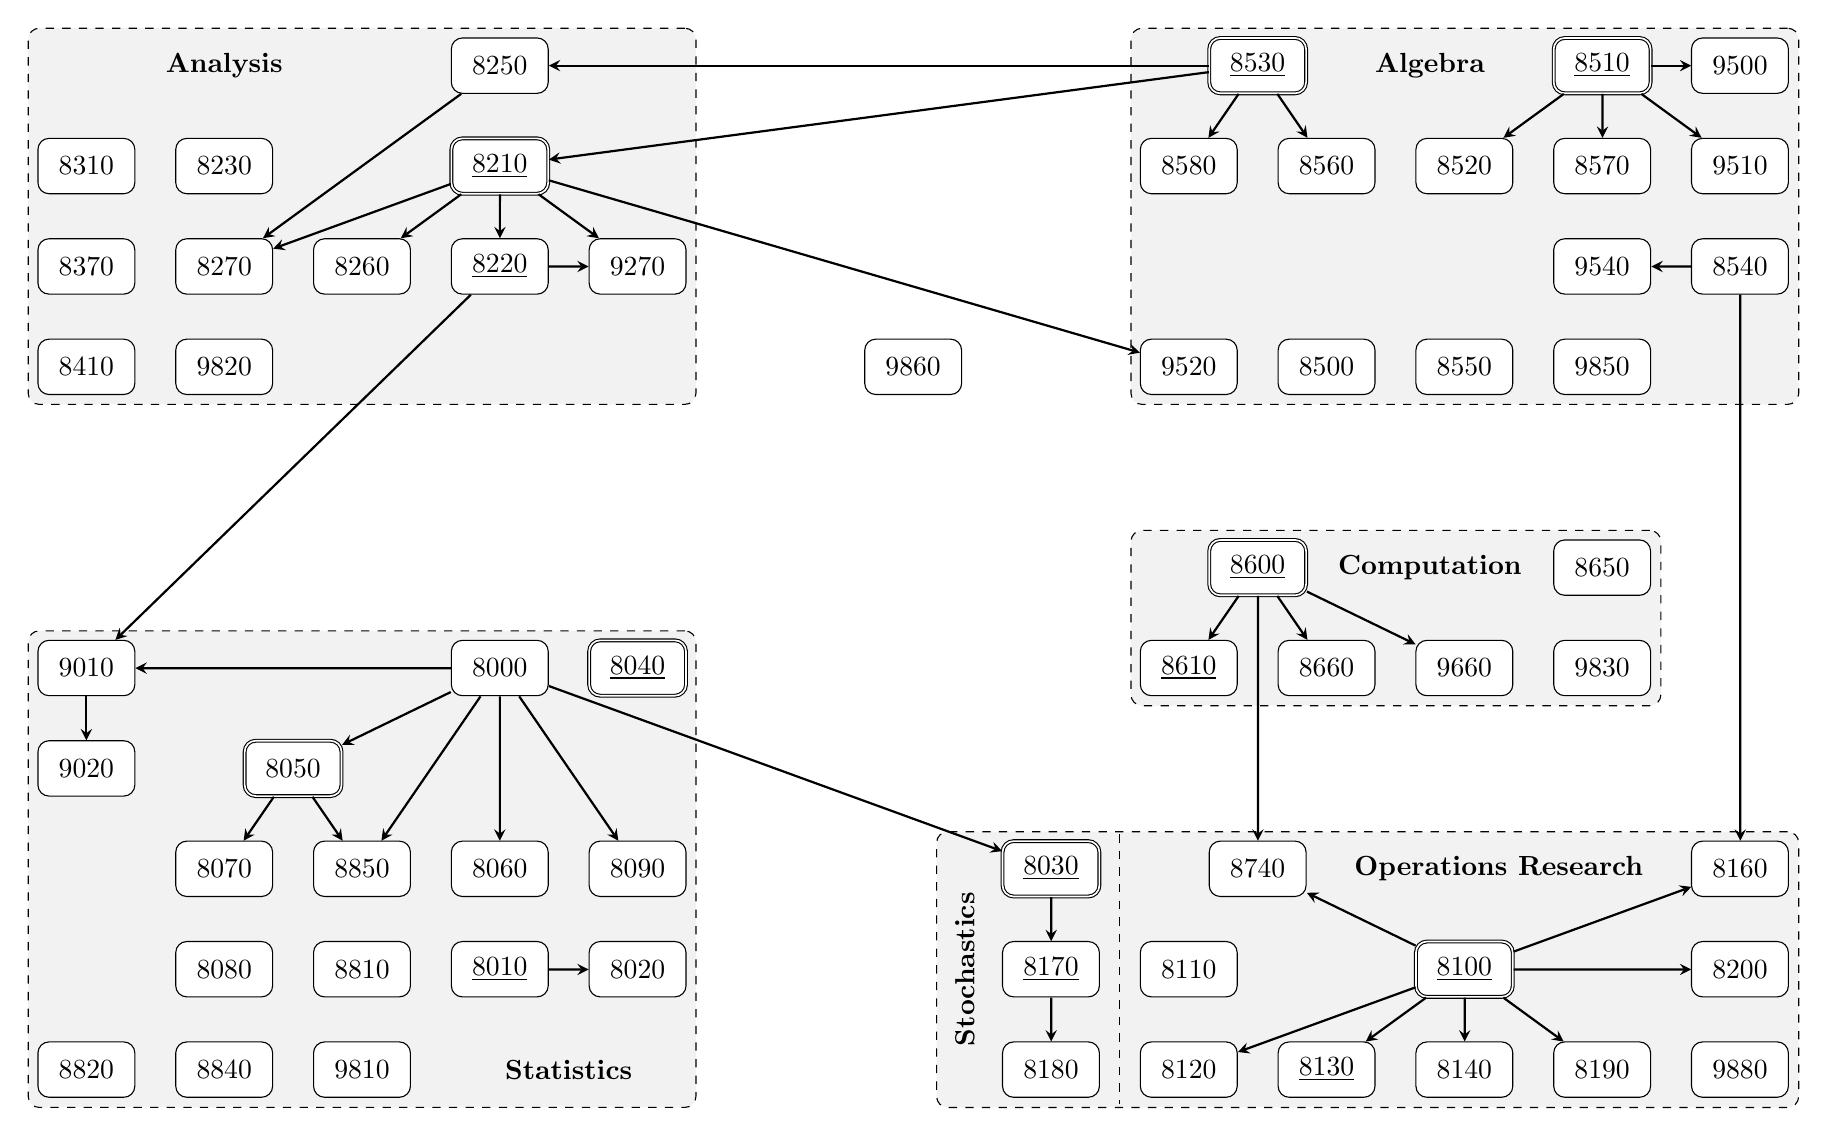
\begin{tikzpicture}[node distance = \nodeHt, xscale =1.75, yscale=1.275]
    %--------------------------------------------------------------------------
    % Analysis
    \node (8310) [class] at (0,  -1) {8310};
    \node (8230) [class] at (1,  -1) {8230};
    \node (8370) [class] at (0,  -2) {8370};
    \node (8270) [class] at (1,  -2) {8270};
    \node (8260) [class] at (2,  -2) {8260};
    \node (9270) [class] at (4,  -2) {9270};
    \node (8210) [class, double] at (3, -1) {\underline{8210}};
    \node (8250) [class] at (3,   0) {8250};
    \node (8410) [class] at (0,  -3) {8410};
    \node (9820) [class] at (1,  -3) {9820};
    \node (8220) [class] at (3,  -2) {\underline{8220}};
    %--------------------------------------------------------------------------
    % Algebra
    \node (8530) [class, double] at (8.5, 0) {\underline{8530}};
    \node (8510) [class, double] at (11,  0) {\underline{8510}};
    \node (9500) [class] at (12,  0) {9500};
    \node (8580) [class] at (8,  -1) {8580};
    \node (8560) [class] at (9,  -1) {8560};
    \node (8520) [class] at (10, -1) {8520};
    \node (8570) [class] at (11, -1) {8570};
    \node (9510) [class] at (12, -1) {9510};
    \node (9540) [class] at (11, -2) {9540};
    \node (8540) [class] at (12, -2) {8540};
    \node (9520) [class] at (8,  -3) {9520};
    \node (8500) [class] at (9,  -3) {8500};
    \node (8550) [class] at (10, -3) {8550};
    \node (9850) [class] at (11, -3) {9850};
    %--------------------------------------------------------------------------
    %Statistics
    \node (9010) [class] at (0,  -6) {9010};
    \node (8000) [class] at (3, -6) {8000};
    \node (8040) [class, double] at (4, -6) {\underline{8040}};
    \node (9020) [class] at (0,  -7) {9020};
    \node (8050) [class, double] at (1.5, -7) {8050};
    \node (8070) [class] at (1,  -8) {8070};
    \node (8850) [class] at (2,  -8) {8850};
    \node (8060) [class] at (3,  -8) {8060};
    \node (8090) [class] at (4,  -8) {8090};
    \node (8080) [class] at (1,  -9) {8080};
    \node (8810) [class] at (2,  -9) {8810};
    \node (8010) [class] at (3,  -9) {\underline{8010}};
    \node (8020) [class] at (4,  -9) {8020};
    \node (8820) [class] at (0, -10) {8820};
    \node (8840) [class] at (1, -10) {8840};
    \node (9810) [class] at (2, -10) {9810};
    %--------------------------------------------------------------------------
    % Computation
    \node (8600) [class, double] at (8.5, -5) {\underline{8600}};
    \node (8650) [class] at (11, -5) {8650};
    \node (8610) [class] at (8,  -6) {\underline{8610}};
    \node (8660) [class] at (9,  -6) {8660};
    \node (9660) [class] at (10,  -6) {9660};
    %\node (8630) [class] at (10, -6) {8630};
    \node (9830) [class] at (11, -6) {9830};
    
    %--------------------------------------------------------------------------
    % Operations Research
    \node (8740) [class] at (8.5,-8) {8740};
    \node (8100) [class, double] at (10, -9) {\underline{8100}};
    \node (8160) [class] at (12, -8) {8160};
    \node (8110) [class] at (8,  -9) {8110};
    \node (8120) [class] at (8, -10) {8120};
    \node (8130) [class] at (9, -10) {\underline{8130}};
    \node (8140) [class] at (10,-10) {8140};
    \node (8190) [class] at (11,-10) {8190};
    \node (8200) [class] at (12, -9) {8200};
    \node (9880) [class] at (12,-10) {9880};
    %--------------------------------------------------------------------------
    % Stochastics
    \node (8030) [class, double] at (7,  -8) {\underline{8030}};
    \node (8170) [class] at (7,  -9) {\underline{8170}};
    \node (8180) [class] at (7, -10) {8180};
    %--------------------------------------------------------------------------
    % Misc
    %% the durp node is magical
    \node (9860) [class] at (6,  -3) {9860};
    %--------------------------------------------------------------------------
    % Subjects titles
    %% titles are positioned relative to class nodes
    \node (analysis)    at (1,     0) {\textbf{Analysis}};
    \node (algebra)     at (9.75,  0) {\textbf{Algebra}};
    \node (stats)       at (3.5, -10) {\textbf{Statistics}};
    \node (comp)        at (9.75, -5) {\textbf{Computation}};
    \node (OR)          at (10.25,-8) {\textbf{Operations Research}};
    \node (stochastics) at (6.375,-9) [rotate=90] {\textbf{Stochastics}};
    %--------------------------------------------------------------------------
    % Subject groupings
    %% rectangles are drawn to fit around other nodes
    %% Could use all nodes in each subject, but I just used enough
    \begin{scope}[on background layer]
      \node (analysisG) [subject, fit=(8250) (9270) (8410)] {};
      \node (algebraG)  [subject, fit=(8580) (9500) (9850)] {};
      \node (statsG)    [subject, fit=(9010) (8040) (8840)] {};
      \node (compG)     [subject, fit=(8600) (8650) (8610)] {};
      \node (orG)       [subject, fit=(8160) (9880) (stochastics)] {};
      %% Dashed line separating OR and Stochastics
      \draw [dashed, shorten >=-12.5pt, shorten <=-12.5pt] (7.5, -8) -- (7.5, -10);
    \end{scope}
    %--------------------------------------------------------------------------
    % Dependencies
    \draw [arrow] (8000) -- (8050);
    \draw [arrow] (8000) -- (8060);
    \draw [arrow] (8000) -- (8090);
    \draw [arrow] (8000) -- (8030); 
    \draw [arrow] (8000) -- (8850);
    \draw [arrow] (8000) -- (9010);
    \draw [arrow] (8010) -- (8020);
    \draw [arrow] (8030) -- (8170);
    \draw [arrow] (8050) -- (8070);
    \draw [arrow] (8050) -- (8850);
    \draw [arrow] (8100) -- (8120);
    \draw [arrow] (8100) -- (8130);
    \draw [arrow] (8100) -- (8140);
    \draw [arrow] (8100) -- (8160);
    \draw [arrow] (8100) -- (8190);
    \draw [arrow] (8100) -- (8200);
    \draw [arrow] (8100) -- (8740);
    \draw [arrow] (8170) -- (8180);
    \draw [arrow] (8210) -- (8220);
    \draw [arrow] (8210) -- (8260);
    \draw [arrow] (8210) -- (8270);
    \draw [arrow] (8210) -- (9270);
    \draw [arrow] (8210) -- (9520);
    \draw [arrow] (8220) -- (9010);
    \draw [arrow] (8220) -- (9270);
    \draw [arrow] (8250) -- (8270);
    \draw [arrow] (8510) -- (8520);
    %\draw [arrow] (8510) -- (8560);
    \draw [arrow] (8510) -- (8570);
    \draw [arrow] (8510) -- (9500);
    \draw [arrow] (8510) -- (9510);
    \draw [arrow] (8530) -- (8210);
    \draw [arrow] (8530) -- (8250);
    \draw [arrow] (8530) -- (8560);
    \draw [arrow] (8530) -- (8580);
    \draw [arrow] (8540) -- (8160);
    \draw [arrow] (8540) -- (9540);
    \draw [arrow] (8600) -- (8610);
    \draw [arrow] (8600) -- (8660);
    \draw [arrow] (8600) -- (9660);
    \draw [arrow] (8600) -- (8740);
    %\draw [arrow] (8630) -- (8160);
    \draw [arrow] (9010) -- (9020);
    %\draw [arrow] () -- ();
  \end{tikzpicture}
  \vspace*{\fill}
\end{document}
%----------------------------------------------------------------
